

%% ,prefix.string=./graph/crv}

%%  LaTeX script for the lecture "Linea and generalized linear models"
%%  in SPE, Saturday 24 August, 2019 -- Esa Läärä

%% \documentclass[12pt,t,dvipsnames,handout% Uncomment ",handout" when doing handouts
%% ]{beamer}

\documentclass[12pt,dvipsnames,t,aspectratio=169 , handout% (Un)comment ",handout" when (not) doing handouts
]{beamer}


\newcommand{\toggle}[1]{%
\addtocounter{framenumber}{-1}#1 % Comment this out if extra slides should be omitted
}
\newcommand{\toggleafter}[1]{%
#1\addtocounter{framenumber}{-1} % Comment this out if extra slides should be omitted
}

\usepackage[latin1]{inputenc}
\usepackage[english]{babel}
\usepackage{booktabs,amsmath,amsbsy,Sweave,relsize}
\usepackage{verbatim}
\usepackage{hyperref}

\usepackage{color}
\usepackage{tikz}

% Tikz settings optimized for causal graphs.
% Just copy-paste this part
\usetikzlibrary{shapes,decorations,arrows,calc,arrows.meta,fit,positioning}
\tikzset{
    -Latex,auto,node distance =1 cm and 1 cm,semithick,
    state/.style ={ellipse, draw, minimum width = 0.7 cm},
    point/.style = {circle, draw, inner sep=0.04cm,fill,node contents={}},
    bidirected/.style={Latex-Latex,dashed},
		dasharrow/.style={Latex, dashed},
    el/.style = {inner sep=2pt, align=left, sloped}
}



%----------------------------------------------------------------------
% The general look of things:

% Theme with navigation bar on the right; [width=0em] removes it
\mode<presentation>{\usetheme[width=0em]{Goettingen}}

% Omit the navigation symbols --- I have pg-up and pg-dn anyway
\setbeamertemplate{navigation symbols}{}

% Pagenumbering at the far right bottom corner
\setbeamertemplate{footline}{
  \usebeamercolor[fg]{frametitle}
  \hspace*{3ex}\currentlecture % This is for inserting title of the
                               % lecture
  \hfill \bf \insertframenumber / \inserttotalframenumber
  \rule[-2ex]{0pt}{5ex} \hspace*{3ex}}

% How visible should the uncovered items be? 0 corresponds to not at all.
\setbeamercovered{transparent=0}

% Get the fonts to look right in mathematics parts
\usefonttheme[onlymath]{serif}
% This is a file of useful extra commands snatched from
% Michael Hills, David Clayton, Bendix Carstensen & Esa Laara.
%

% Commands to draw observation lines on follow-up diagrams
%
% Horizontal lines
%

% exit time with failure, bullet
\newcommand{\hfail}[1]{\begin{picture}(250,5)
       \put(0,0){\line(0,1){2.5}}
      \put(0,0){\line(0,-1){2.5}}
      \put(0,0){\line(1,0){#1}}
      \put(#1,0){\circle*{5}}
   \end{picture}}

% exit time with censoring, open circle
\newcommand{\hcens}[1]{\begin{picture}(250,5)
         \put(0,0){\line(0,1){2.5}}
      \put(0,0){\line(0,-1){2.5}}
      \put(0,0){\line(1,0){#1}}
%      \put(#1,0){\line(0,1){2.5}}
%      \put(#1,0){\line(0,-1){2.5}}
% BxC Changed this to an open circle instead of a line
      \put(#1,0){\circle{5}}
   \end{picture}}

%
% Diagonals for Lexis diagrams
%
\newcommand{\dfail}[1]{\begin{picture}(250,250)
      \put(0,0){\line(1,1){#1}}
      \put(#1,#1){\circle*{5}}
   \end{picture}}

\newcommand{\dcens}[1]{\begin{picture}(250,250)
      \put(0,0){\line(1,1){#1}}
%      \put(#1,#1){\line(0,1){2.5}}
%      \put(#1,#1){\line(0,-1){2.5}}
% BxC Changed this to an open circle instead of a line
      \put(#1,#1){\circle{5}}
   \end{picture}}

%
% Horizontal range diagrams
%
\newcommand{\hrange}[1]{\begin{picture}(200,5)
     \put(0,0){\circle*{5}}
     \put(0,0){\line(1,0){#1}}
     \put(0,0){\line(-1,0){#1}}
   \end{picture}}

%
% Tree drawing
%
\newcommand{\tree}[3]{\setlength{\unitlength}{#1}\begin{picture}(0,0)
   \put(0,0){\line(3,2){1}}
   \put(0,0){\line(3,-2){1}}
   \put(0.81,0.54){\makebox(0,0)[br]{\footnotesize #2\ }}
   \put(0.81,-0.54){\makebox(0,0)[tr]{\footnotesize #3\ }}
\end{picture}}

\newcommand{\wtree}[3]{\setlength{\unitlength}{#1}\begin{picture}(0,0)
   \put(0,0){\line(1,1){1}}
   \put(0,0){\line(1,-1){1}}
   \put(0.8,0.8){\makebox(0,0)[br]{\footnotesize #2\ }}
   \put(0.8,-0.8){\makebox(0,0)[tr]{\footnotesize #3\ }}
\end{picture}}

\newcommand{\ntree}[3]{\setlength{\unitlength}{#1}\begin{picture}(0,0)
   \put(0,0){\line(2,1){1}}
   \put(0,0){\line(2,-1){1}}
   \put(0.8,0.4){\makebox(0,0)[br]{\footnotesize #2\ }}
   \put(0.8,-0.4){\makebox(0,0)[tr]{\footnotesize #3\ }}
\end{picture}}

%
% Other commands
%
\newcommand{\T}{\scriptsize\text T}
\newcommand{\prob}[0]{\text{\rm Pr}}
\newcommand{\nhy}[0]{_{\oslash}}
\newcommand{\true}[0]{_{\text{\rm \tiny T}}}
\newcommand{\hyp}[0]{_{\text{\rm \tiny H}}}
% \newcommand{\mpydiv}[0]{\stackrel{\textstyle \times}{\div}}
% Changed to slightly smaller symbols
\newcommand{\mpydiv}[0]{\stackrel{\times}{\scriptstyle \div}}
\newcommand{\mie}[1]{{\it #1}}
\newcommand{\mycircle}[0]{\circle*{5}}
\newcommand{\smcircle}[0]{\circle*{1}}
\newcommand{\corner}[0]{_{\text{\rm \tiny C}}}
\newcommand{\ind}[0]{\hspace{10pt}}
\newcommand{\gap}[0]{\\[5pt]}
\renewcommand{\S}[0]{section~}
\newcommand{\blank}[0]{$\;\,$}
\newcommand{\vone}{\vspace{1cm}}
\newcommand{\ljust}[1]{\multicolumn{1}{l}{#1}}
\newcommand{\cjust}[1]{\multicolumn{1}{c}{#1}}
\newcommand{\mean}{\text{\rm Mean}}
\newcommand{\transpose}{^{\mbox{\tiny T}}}
\newcommand{\histog}[5]{\rule{1mm}{#1mm}\,\rule{1mm}{#2mm}\,\rule{1mm}{#3mm}\,\rule{1mm}{#4mm}\,\rule{1mm}{#5mm}}
\newcommand{\pmiss}{P_{\mbox{\tiny miss}}}
%
% Below is BxCs commands inserted
%
\newcommand{\bc}{\begin{center}}
\newcommand{\ec}{\end{center}}

\newcommand{\bd}{\setlength{\parskip}{1ex} \begin{description}}
\newcommand{\ed}{\end{description} \setlength{\parskip}{2ex}}
\newcommand{\bdx}{\begin{description}} % Bendix' description macros
\newcommand{\edx}{\end{description}}

\newcommand{\bix}{\begin{itemize}}  % these are Bendix' itemizing macros
\newcommand{\eix}{\end{itemize}}
\newcommand{\bi}{\setlength{\parskip}{1ex} \begin{itemize}} % Esa's item macros 
\newcommand{\ei}{\end{itemize} \setlength{\parskip}{2ex}} 

\newcommand{\bn}{\begin{equation}}
\newcommand{\en}{\end{equation}}
\newcommand{\be}{\begin{enumerate}}
\newcommand{\ee}{\end{enumerate}}
\newcommand{\bes}{\begin{eqnarray*}}
\newcommand{\ees}{\end{eqnarray*}}
\newcommand{\p}{\text{\rm P}}
\newcommand{\pmat}[1]{\text{\rm P}\left\{#1\right\}}
\newcommand{\ptxt}[1]{\text{\rm P}\left\{\text{\rm #1}\right\}}
\newcommand{\E}{\text{\rm E}}
\newcommand{\V}{\text{\rm V}}
\newcommand{\BLUP}{\text{\rm BLUP}}

% \newcommand{\var}{\mbox{Var}} changed by Esa to
\newcommand{\var}{\mbox{var}}
% \newcommand{\cov}{\mbox{Cov}} changed by Esa to
\newcommand{\cov}{\mbox{cov}}
% \newcommand{\corr}{\mbox{Corr}} changed by Esa to
\newcommand{\corr}{\mbox{corr}} 

%\newcommand{\var}{\text{\rm var}}
%\newcommand{\cov}{\text{\rm cov}}
%\newcommand{\corr}{\text{\rm corr}}
\newcommand{\se}{\text{\rm s.e.}}
\newcommand{\sd}{\text{\rm std}}
\newcommand{\erf}{\text{\rm erf}}
\newcommand{\odds}{\text{\rm odds}}
\newcommand{\bin}{\text{\rm binom}}
\newcommand{\half}[1]{\frac{1}{#1}}
% \newcommand{\td}[0]{\stackrel{\textstyle \times}{\div}}
% Changed to slightly smaller symbols
\newcommand{\td}[0]{\stackrel{\scriptstyle \times}{\scriptstyle \div}}
\newcommand{\logit}{\text{\rm logit}}
\newcommand{\link}{\text{\rm link}}
\newcommand{\spn}{\text{\rm span}}
\newcommand{\OR}{\text{\rm OR}}
\newcommand{\RR}{\text{\rm RR}}
\newcommand{\ER}{\text{\rm ER}}
\newcommand{\RD}{\text{\rm RD}}
\newcommand{\AC}{\text{\rm AC}}
\newcommand{\AF}{\text{\rm AF}}
\newcommand{\PAF}{\text{\rm PAF}}
\newcommand{\SR}{\text{\rm SR}}
\newcommand{\SMR}{\text{\rm SMR}}
\newcommand{\CMF}{\text{\rm CMF}}
\newcommand{\pvp}{\text{\rm PV}$+$}
\newcommand{\pvn}{\text{\rm PV}$-$}
\newcommand{\R}{\textsf{R}}
%\newcommand{\gap}[0]{\\[5pt]} 
%\newcommand{\blank}[0]{$\;\,$}
% Conditional independence sign from Philip Dawid
\newcommand{\cip}{\mbox{$\perp\!\!\!\perp$}}

%%% Commands to comment out parts of the text
\newcommand{\GLEM}[1]{}
\newcommand{\FORGETIT}[1]{}
\newcommand{\OMIT}[1]{}

%%% Insert output from program in small text 
%%% (requires package verbatim)

\newcommand{\insout}[1]{
\scriptsize
\renewcommand{\baselinestretch}{0.8}
\verbatiminput{#1}
\renewcommand{\baselinestretch}{1.0}
\normalsize
}

% From Esa:        
%\newcommand{\T}{\text{\rm \small{T}}}
\newcommand{\id}{\text{\rm id}}
\newcommand{\Dev}{\text{\rm Dev}}
\newcommand{\Bin}{\text{\rm Bin}}
\newcommand{\probit}{\text{\rm probit}}
\newcommand{\cloglog}{\text{\rm cloglog}}
\newcommand{\EF}{\text{\rm EF}}
\newcommand{\SE}{\text{\rm SE}}
\newcommand{\IP}{\text{\rm IP}}



% % This is a file of redefinitions of the mathematical functions
% so that they can be typeset in serif font in Beamer
\renewcommand{\arccos}[0]{\text{\rm arccos}}
\renewcommand{\arcsin}[0]{\text{\rm arcsin}}
\renewcommand{\arctan}[0]{\text{\rm arctan}}
\renewcommand{\arg}[0]{\text{\rm arg}}
\renewcommand{\cos}[0]{\text{\rm cos}}
\renewcommand{\cosh}[0]{\text{\rm cosh}}
\renewcommand{\cot}[0]{\text{\rm cot}}
\renewcommand{\coth}[0]{\text{\rm coth}}
\renewcommand{\csc}[0]{\text{\rm csc}}
\renewcommand{\deg}[0]{\text{\rm deg}}
\renewcommand{\det}[0]{\text{\rm det}}
\renewcommand{\dim}[0]{\text{\rm dim}}
\renewcommand{\exp}[0]{\text{\rm exp}}
\renewcommand{\gcd}[0]{\text{\rm gcd}}
\renewcommand{\hom}[0]{\text{\rm hom}}
\renewcommand{\inf}[0]{\text{\rm inf}}
\renewcommand{\ker}[0]{\text{\rm ker}}
\renewcommand{\lg}[0]{\text{\rm lg}}
\renewcommand{\lim}[0]{\text{\rm lim}}
\renewcommand{\liminf}[0]{\text{\rm liminf}}
\renewcommand{\limsup}[0]{\text{\rm limsup}}
\renewcommand{\ln}[0]{\text{\rm ln}}
\renewcommand{\log}[0]{\text{\rm log}}
\renewcommand{\max}[0]{\text{\rm max}}
\renewcommand{\min}[0]{\text{\rm min}}
\renewcommand{\Pr}[0]{\text{\rm Pr}}
\renewcommand{\sec}[0]{\text{\rm sec}}
\renewcommand{\sin}[0]{\text{\rm sin}}
\renewcommand{\sinh}[0]{\text{\rm sinh}}
\renewcommand{\sup}[0]{\text{\rm sup}}
\renewcommand{\tan}[0]{\text{\rm tan}}
\renewcommand{\tanh}[0]{\text{\rm tanh}}

% Extra functions in math style
\newcommand{\pr}[0]{\text{\rm Pr}}
\newcommand{\var}{\text{\rm var}}
\newcommand{\cov}{\text{\rm cov}}
\newcommand{\corr}{\text{\rm corr}}
\newcommand{\mean}{\text{\rm mean}}
\newcommand{\median}{\text{\rm median}}
\newcommand{\p}{{\mathrm p}}
\newcommand{\e}{{\mathrm e}}
\newcommand{\D}{{\mathrm D}}
\newcommand{\dif}{{\,\mathrm d}}
% \newcommand{\Pp}{P}
\newcommand{\pmat}[1]{\Pp\left\{#1\right\}}
\newcommand{\ptxt}[1]{\Pp\left\{\text{#1}\right\}}
% \newcommand{\pmat}[1]{\text{\rm P}\left\{#1\right\}}
% \newcommand{\ptxt}[1]{\text{\rm P}\left\{\text{#1}\right\}}
\newcommand{\E}{\text{\rm E}}
\newcommand{\V}{\text{\rm V}}
\newcommand{\BLUP}{\text{\rm BLUP}}
\newcommand{\se}{\text{\rm s.e.}}
\newcommand{\sem}{\text{\rm s.e.m.}}
\newcommand{\std}{\text{\rm std}}
\newcommand{\sd}{\text{\rm s.d.}}
\newcommand{\cv}{\text{\rm c.v.}}
\newcommand{\CV}{\text{\rm CV}}
\newcommand{\erf}{\text{\rm erf}}
\newcommand{\ef}{\text{\rm ef}}
\newcommand{\SSD}{\text{\rm SSD}}
\newcommand{\SPD}{\text{\rm SPD}}
\newcommand{\odds}{\text{\rm odds}}
\newcommand{\bin}{\text{\rm binom}}
\newcommand{\diag}{\text{\rm diag}}
\newcommand{\spcol}{\text{\rm span}}
\newcommand{\logit}{\text{\rm logit}}
% Intentional typo to avoid name conflict
\newcommand{\lnik}{\text{\rm link}}
\newcommand{\spn}{\text{\rm span}}
\newcommand{\CI}{\text{\rm CI}}
\newcommand{\IP}{\text{\rm IP}}
\newcommand{\OR}{\text{\rm OR}}
\newcommand{\RR}{\text{\rm RR}}
\newcommand{\ER}{\text{\rm ER}}
\newcommand{\EM}{\text{\rm EM}}
\newcommand{\EF}{\text{\rm EF}}
\newcommand{\RD}{\text{\rm RD}}
\newcommand{\AC}{\text{\rm AC}}
\newcommand{\AF}{\text{\rm AF}}
\newcommand{\PAF}{\text{\rm PAF}}
\newcommand{\AR}{\text{\rm AR}}
\newcommand{\CR}{\text{\rm CR}}
\newcommand{\PAR}{\text{\rm PAR}}
\newcommand{\SD}{\text{\rm SD}}
\newcommand{\SE}{\text{\rm SE}}
\newcommand{\SEM}{\text{\rm SEM}}
\newcommand{\SR}{\text{\rm SR}}
\newcommand{\SMR}{\text{\rm SMR}}
\newcommand{\RSR}{\text{\rm RSR}}
\newcommand{\CMF}{\text{\rm CMF}}
\newcommand{\pvp}{\text{\rm PV$+$}}
\newcommand{\pvn}{\text{\rm PV$-$}}
\newcommand{\T}{\text{\rm \small{T}}}
\newcommand{\id}{\text{\rm id}}
\newcommand{\Dev}{\text{\rm Dev}}
\newcommand{\Bin}{\text{\rm Bin}}
\newcommand{\probit}{\text{\rm probit}}
\newcommand{\cloglog}{\text{\rm cloglog}}

% Conditional independence sign from Philip Dawid
\newcommand{\cip}{\mbox{$\perp\!\!\!\perp$}}
\newcommand{\half}{\frac{1}{2}}
% Multoply / division
\newcommand{\mpydiv}[0]{\stackrel{\scriptstyle \times}{\scriptstyle \div}}
\newcommand{\td}[0]{\stackrel{\scriptstyle \times}{\scriptstyle \div}}
\newcommand{\dt}[0]{\stackrel{\scriptstyle \div}{\scriptstyle \times}}

%% % This is a file of redefinitions of the mathematical functions
% so that they can be typeset in serif font in Beamer
\renewcommand{\arccos}[0]{\text{\rm arccos}}
\renewcommand{\arcsin}[0]{\text{\rm arcsin}}
\renewcommand{\arctan}[0]{\text{\rm arctan}}
\renewcommand{\arg}[0]{\text{\rm arg}}
\renewcommand{\cos}[0]{\text{\rm cos}}
\renewcommand{\cosh}[0]{\text{\rm cosh}}
\renewcommand{\cot}[0]{\text{\rm cot}}
\renewcommand{\coth}[0]{\text{\rm coth}}
\renewcommand{\csc}[0]{\text{\rm csc}}
\renewcommand{\deg}[0]{\text{\rm deg}}
\renewcommand{\det}[0]{\text{\rm det}}
\renewcommand{\dim}[0]{\text{\rm dim}}
\renewcommand{\exp}[0]{\text{\rm exp}}
\renewcommand{\gcd}[0]{\text{\rm gcd}}
\renewcommand{\hom}[0]{\text{\rm hom}}
\renewcommand{\inf}[0]{\text{\rm inf}}
\renewcommand{\ker}[0]{\text{\rm ker}}
\renewcommand{\lg}[0]{\text{\rm lg}}
\renewcommand{\lim}[0]{\text{\rm lim}}
\renewcommand{\liminf}[0]{\text{\rm liminf}}
\renewcommand{\limsup}[0]{\text{\rm limsup}}
\renewcommand{\ln}[0]{\text{\rm ln}}
\renewcommand{\log}[0]{\text{\rm log}}
\renewcommand{\max}[0]{\text{\rm max}}
\renewcommand{\min}[0]{\text{\rm min}}
\renewcommand{\Pr}[0]{\text{\rm Pr}}
\renewcommand{\sec}[0]{\text{\rm sec}}
\renewcommand{\sin}[0]{\text{\rm sin}}
\renewcommand{\sinh}[0]{\text{\rm sinh}}
\renewcommand{\sup}[0]{\text{\rm sup}}
\renewcommand{\tan}[0]{\text{\rm tan}}
\renewcommand{\tanh}[0]{\text{\rm tanh}}

% Extra functions in math style
\newcommand{\pr}[0]{\text{\rm Pr}}
\newcommand{\var}{\text{\rm var}}
\newcommand{\cov}{\text{\rm cov}}
\newcommand{\corr}{\text{\rm corr}}
\newcommand{\mean}{\text{\rm mean}}
\newcommand{\median}{\text{\rm median}}
\newcommand{\p}{{\mathrm p}}
\newcommand{\e}{{\mathrm e}}
\newcommand{\D}{{\mathrm D}}
\newcommand{\dif}{{\,\mathrm d}}
% \newcommand{\Pp}{P}
\newcommand{\pmat}[1]{\Pp\left\{#1\right\}}
\newcommand{\ptxt}[1]{\Pp\left\{\text{#1}\right\}}
% \newcommand{\pmat}[1]{\text{\rm P}\left\{#1\right\}}
% \newcommand{\ptxt}[1]{\text{\rm P}\left\{\text{#1}\right\}}
\newcommand{\E}{\text{\rm E}}
\newcommand{\V}{\text{\rm V}}
\newcommand{\BLUP}{\text{\rm BLUP}}
\newcommand{\se}{\text{\rm s.e.}}
\newcommand{\sem}{\text{\rm s.e.m.}}
\newcommand{\std}{\text{\rm std}}
\newcommand{\sd}{\text{\rm s.d.}}
\newcommand{\cv}{\text{\rm c.v.}}
\newcommand{\CV}{\text{\rm CV}}
\newcommand{\erf}{\text{\rm erf}}
\newcommand{\ef}{\text{\rm ef}}
\newcommand{\SSD}{\text{\rm SSD}}
\newcommand{\SPD}{\text{\rm SPD}}
\newcommand{\odds}{\text{\rm odds}}
\newcommand{\bin}{\text{\rm binom}}
\newcommand{\diag}{\text{\rm diag}}
\newcommand{\spcol}{\text{\rm span}}
\newcommand{\logit}{\text{\rm logit}}
% Intentional typo to avoid name conflict
\newcommand{\lnik}{\text{\rm link}}
\newcommand{\spn}{\text{\rm span}}
\newcommand{\CI}{\text{\rm CI}}
\newcommand{\IP}{\text{\rm IP}}
\newcommand{\OR}{\text{\rm OR}}
\newcommand{\RR}{\text{\rm RR}}
\newcommand{\ER}{\text{\rm ER}}
\newcommand{\EM}{\text{\rm EM}}
\newcommand{\EF}{\text{\rm EF}}
\newcommand{\RD}{\text{\rm RD}}
\newcommand{\AC}{\text{\rm AC}}
\newcommand{\AF}{\text{\rm AF}}
\newcommand{\PAF}{\text{\rm PAF}}
\newcommand{\AR}{\text{\rm AR}}
\newcommand{\CR}{\text{\rm CR}}
\newcommand{\PAR}{\text{\rm PAR}}
\newcommand{\SD}{\text{\rm SD}}
\newcommand{\SE}{\text{\rm SE}}
\newcommand{\SEM}{\text{\rm SEM}}
\newcommand{\SR}{\text{\rm SR}}
\newcommand{\SMR}{\text{\rm SMR}}
\newcommand{\RSR}{\text{\rm RSR}}
\newcommand{\CMF}{\text{\rm CMF}}
\newcommand{\pvp}{\text{\rm PV$+$}}
\newcommand{\pvn}{\text{\rm PV$-$}}
\newcommand{\T}{\text{\rm \small{T}}}
\newcommand{\id}{\text{\rm id}}
\newcommand{\Dev}{\text{\rm Dev}}
\newcommand{\Bin}{\text{\rm Bin}}
\newcommand{\probit}{\text{\rm probit}}
\newcommand{\cloglog}{\text{\rm cloglog}}

% Conditional independence sign from Philip Dawid
\newcommand{\cip}{\mbox{$\perp\!\!\!\perp$}}
\newcommand{\half}{\frac{1}{2}}
% Multoply / division
\newcommand{\mpydiv}[0]{\stackrel{\scriptstyle \times}{\scriptstyle \div}}
\newcommand{\td}[0]{\stackrel{\scriptstyle \times}{\scriptstyle \div}}
\newcommand{\dt}[0]{\stackrel{\scriptstyle \div}{\scriptstyle \times}}
 % A re-definition of all math
                        % commands (and some more) that
                        % makes them appear in serif font

% The heading font is a little too thin to my taste
\setbeamerfont{frametitle}{size=\large,series=\bfseries}

% Use pdf graphs
\DeclareGraphicsExtensions{.pdf,.jpg,.jpeg}

% End of setting up the formal layout of the slides

% Definition of a dummy command so that the above works and so that ALL
% redefinitions can be done by \renewcommand{\currentlecture}
\newcommand{\currentlecture}{}

% A banner page to include and separate lectures
\newcommand{\banner}[4]{
\addtocounter{framenumber}{-1}
\section{#1}
\renewcommand{\currentlecture}{#1}
\begin{frame}[plain]
{\usebeamercolor[fg]{frametitle}
 \LARGE \bf #1\\[1ex]
 \large \sf #2\\
 \large \bf #3}
\vfill
Statistical Practice in Epidemiology with \textbf{R}\\
2 to 7 June, 2023\\
University of Tartu, Estonia
%% International Agency for Research on Cancer, Lyon, France
\end{frame}
\input{#4}
}

% % PD additions
% \usepackage[T1]{fontenc}
% \usepackage{moreverb}
% \newcommand{\code}[1]{\texttt{#1}}
% \let\overbatim\verbatim
% \let\endoverbatim\endverbatim
% \newenvironment{vcode}%
% {\bgroup\baselineskip=0.8\baselineskip\overbatim}%
% {\endoverbatim\egroup}

% MP additions
\newcommand{\code}[1]{\texttt{\color{blue}#1}}
\newcommand{\comma}{{\color{black},}}
\newcommand{\Rarrow}{{\color{green}<-}}
\newcommand{\Rprompt}{{\color{black}>~}}
\newcommand{\Rcont}{{\color{black}+~}}
\newcommand{\Rc}{{\color{black},}}
\newcommand{\RT}{{\color{green}TRUE}}
\newcommand{\RF}{{\color{green}FALSE}}
\newcommand{\Rcomment}[1]{{\color{brown}\##1}}
\newcommand{\indep}{\perp\!\!\!\perp}
\newcommand{\depend}{\not\!\perp\!\!\!\perp}

%----------------------------------------------------------------------
\begin{document}
% It is more readable with a little extra space between paragraphs
\parskip 0.8ex

% \AtBeginSubsection[]
% {
%   \begin{frame}<beamer>
%     \frametitle{Outline}
%     \tableofcontents[currentsection,currentsubsection]
%   \end{frame}
% }
% \beamerdefaultoverlayspecification{<+->}

% %----------------------------------------------------------------------
% % The default titlepage is horribly formatted, so a custom made one:
% \addtocounter{framenumber}{-1}
% \begin{frame}[plain]
% {\usebeamercolor[fg]{frametitle}
%  \LARGE \bf Statistical Practice in Epidemiology with R}
% \vfill
% {\scriptsize
%  \bf Bendix Carstensen\sf, Steno Diabetes Center, Copenhagen\\%[1ex]
%  \bf Peter Dalgaard\sf, Dept. of Biostatistics, University of Copenhagen\\%[1ex]
%  \bf Krista Fischer\sf, Dept. of Biostatistics, University of Tartu\\%[1ex]
% %\bf Lyle Gurrin\sf, School of Population Health, University of Melbourne\\%[1ex]
% %\bf Michael Hills\sf, (retired), Highgate, London\\%[1ex]
%  \bf Esa L??r?\sf, Dept. of Mathematics, University of Oulu\\%[1ex]
%  \bf Martyn Plummer\sf, IARC, Lyon\\%[1ex]
% }
% \normalsize
% \vfill
% June, 2010\\
% Department of Mathematical Statistics,\\ University of Tartu, Estonia.
% \end{frame}

\banner{Causal Inference 2: Model-based estimation of causal contrasts}
       {Tuesday, 6 June, 2023}
       {Esa L{\"a}{\"a}r{\"a}}
      %% {lin-mod}
			
			


\begin{frame}
\frametitle{Outline}

\begin{itemize}

\item Causal questions
\medskip
\item Factual risks and associational contrasts 
\medskip
\item Causal estimands: contrasts of counterfactual quantities
\medskip
\item Marginal and conditional contrasts, effect among treated, etc.
\medskip
\item Outcome regression models, standardization or g-formula
\medskip
\item Exposure modelling, propensity scores and weighting 
\medskip
\item Double robust estimators and machine learning algorithms
\medskip
\item Time-to-event outcomes: hazards of hazard ratios and estimation
of causal contrasts of cumulative risks. 

\end{itemize}

\end{frame}

\begin{frame}
\frametitle{\large Some literature}
\bi
\item \href{https://doi.org/10.1002/sim.6607}{\color{blue}Austin \& Stuart (2015)} {\it Stat Med} 34(28):3661-3679.
\medskip 
\item
\href{https://doi.org/10.1093/aje/kwq439}{\color{blue} Funk et al. (2011)} {\it Am J Epidemiol}  173(7):761-767
\medskip
\item
\href{https://www.hsph.harvard.edu/miguel-hernan/causal-inference-book/}
{\color{blue}Hernan \& Robins (2020)}. \textit{Causal Inference: What if}.
CRC Press.
\medskip
\item
\href{https://doi.org/10.1002/sim.7628}{\color{blue}Luque Fernandez et al. (2018)}
{\it Stat Med} 2018;37(16):2530-2546
\medskip
\item
\href{https://doi.org/10.1093/aje/kww165}{\color{blue}Schuler \& Rose (2017)} \textit{Am J Epidemiol} 185(1):65-73.
\medskip
\item 
 \href{https://doi.org/10.1007/s10654-016-0157-3}{\color{blue}Sj{\"o}lander (2016)} {\it Eur J Epidemiol} 31:563-574
\medskip
\item
\href{https://doi.org/10.1002/sim.9234}{\color{blue}Smith et al. (2022)} {\it Stat Med} 2022;41(2):407-432.
\medskip
\item
\href{https://cran.r-project.org/web/packages/PSweight/vignettes/vignette.pdf}{\color{blue}Zhou et al. (2022)} \texttt{PSweight} vignette.

\ei

\end{frame}

\begin{frame}
\frametitle{Causal question in PECOT format \& Example}

\begin{itemize}
\item[P] \textbf{Population}: 2900 women with breast cancer (Rotterdam study) 
\medskip
\item[E] \textbf{Exposure}: Hormonal treatment (HT)
\medskip
\item[C] \textbf{Comparator}: Placebo, no HT
\medskip
\item[O] \textbf{Outcome}: Recurrence or death
\medskip
\item[T] \textbf{Time frame}: 10 y from surgery to outcome
\end{itemize}

\pause

Causal questions of interest -- comparisons of counterfactuals:

\begin{itemize}
\item[--] What is the 10-year risk $\pi^1$ of the outcome,
\underline{if everybody in P were exposed} to HT, as compared with $\pi^0$, the risk
\underline{if nobody} were exposed?
\pause
\medskip
\item[--] What is the 10-year risk $\pi^1_1$ of the outcome,
\underline{among those in P,} \underline{who are factually exposed} to HT, as compared with the risk $\pi^0_1$, \\
\underline{if they were not} exposed?
\end{itemize}


\end{frame}

\begin{frame}
\frametitle{\large Risks by factual exposure and their associational contrasts}
 
\begin{itemize}
\item
Let %% $T$ = time to outcome event,  
 $Y$ %% (t) = {\mathbf 1}_{\{T \leq t\}}$
 be a binary indicator (1/0)
for the outcome to occur within fixed risk period (assuming no censoring, nor competing events), 
and \\ $X$ be an exposure variable or risk factor. 
\pause
\medskip
\item
Let $\pi_x$ = risk of the outcome to occur during the period in the
\underline{subset of the target population factually exposed} to level $X=x$:
$$ \pi_x = P \{ Y=1\mid X=x\} = E(Y|X=x) . $$
\pause
\item
For simplicity, let $X$ be binary, too: exposed vs. unexposed . %
%% \& suppress dependence on time, too. Assume also absence of competing events.
\pause
\medskip
\item
Common \textbf{associational contrasts}
of risks  between exposure groups:
\medskip
\begin{itemize}
{\normalsize
\item[--] \textbf{Risk difference} $\tau = \pi_1 - \pi_0 = E(Y|X=1) - E(Y|X=0)$,  
% \medskip
\item[--] \textbf{Risk ratio} 
$\phi = {\displaystyle \pi_1}/{\displaystyle \pi_0}$,
% \medskip
\item[--] \textbf{Risk odds ratio} $\psi 
= \frac{\displaystyle \omega_1}{\displaystyle \omega_0} = 
\frac{\displaystyle \pi_1/(1-\pi_1)}
       {\displaystyle \pi_0/(1-\pi_0)}$.
}
\end{itemize}
\end{itemize}
\end{frame}




\begin{frame}
\frametitle{\large Conditional associational contrasts}

\bi
\item
The associational quantities above were \textbf{marginal}; 
not conditioned on \\ (or stratified by) any \textbf{covariate} -- such as sex, age, etc.
\pause
\medskip
\item
Let now $Z$ be a covariate (can be multivariable)  and
$$ \pi_{xz} = P\{ Y=1 \mid  X=x, Z=z \} = E(Y|X=x, Z=z) $$  
be the risk of outcome during risk period in a population group where \\
both $X=x$ \underline{and} $Z=z$, $x=0,1$.
\pause
\medskip
\item
%% Let $\theta$ be any type of marginal associational contrast, and $\theta_z$ 
%% be the analogous
 {\bf Conditional associational contrasts} 
between exposed and unexposed among those with $Z=z$.
\bi
{\normalsize
\item[--]
  $ \tau_z = \pi_{1z} - \pi_{0z}$ is the risk difference conditional on $Z=z$, i.e. {\bf $z$-specific} risk difference. 
\pause	
\medskip
\item[--]
$\phi_z = \pi_{1z}/\pi_{0z}$ and $\psi_z = \pi_{1z}(1-\pi_{1z})/[\pi_{0z}(1 - \pi_{0z})]$ are the  \\ $z$-specific risk ratio and odds ratio, respectively.
}
\ei
%%\medskip
%% \item
%% Conditional contrasts of hazards: $\delta_z = \lambda_{1z}-\lambda_{0z}$ and $\rho_z =  \lambda_{1z}/\lambda_{0z}$,
%% where $\lambda_{xz} = \lambda_{xz}(t) = \lambda(t | X=x, Z=z)$. 
% and those of prevalences, too,
% are defined in an analogous way. 

\ei 
\end{frame}

\begin{frame}
\frametitle{\large Example: Single binary covariate $Z$}

\bi
\item Let the prevalence of exposure be $P\{ X=1 \}$ = 0.45 in the population
\medskip
\item Let % $Z$  
$P\{ Z=1 \} = 1 - P\{ Z=0 \}$ = 0.40 in the population and 
\begin{center}
%% $P\{ X=1|Z=1\}=$ 0.75 and $P\{ X=1| Z=0\}$ = 0.25 $\Rightarrow$ \\
 $P\{ Z=1|X=1\}=$ 0.667 \ and \ $P\{ Z=1| X=0\}$ = 0.182 
\end{center}
\pause
\medskip
\item Let also factual  risks $\pi_{xz} = P\{ Y=1|X=x, Z=z\}$ ($x,z=0,1$) \\
 by $X$ and $Z$ be as shown in the cells of the table below : 
\begin{center}
{\small
\begin{tabular}{l r r l}
\toprule
      & $Z=1$ & $Z=0$ & $\pi_x$ (obtained by formula of total probability) \\
\midrule						
$X=1$ & 0.50  & 0.20 & $\pi_1$ = \textbf{0.40} (0.50$\times$ 0.667 + 0.20$\times$ 0.333) \\
$X=0$ & 0.25  & 0.10 & $\pi_0$ = \textbf{0.13} (0.25$\times$ 0.182 + 0.10$\times$ 0.818) \\
\midrule
Contrasts & $\tau_1$ =0.25 & $\tau_0$ = 0.10 & $\tau$ = \textbf{0.27} \\
\bottomrule  
\end{tabular}
}
\end{center}
\pause
\medskip
\item % [$\Rightarrow$]
 Marginal risks,
$\pi_1, \pi_0$,  contrast $\tau = \pi_1 - \pi_0$,
and conditional contrasts 
$\tau_z = \pi_{1z} - \pi_{0z}$ are shown in table margins.
\ei

\end{frame}


\begin{frame}
\frametitle{\large Associational and causal contrasts}

\begin{center}
\includegraphics[height=4cm, width=7cm]{hernan-jech-2004}
\end{center}
\pause
\bi
\item
\textbf{Associational}: Contrast of risks between the {\bf subsets} of the population 
determined by the subjects' {\bf factual} exposure value.
\pause
\medskip
\item
\textbf{Causal}: Contrast of risks in the {\bf entire population} under the \\ alternative {\bf potential} or {\bf counterfactual} exposure values; \\ 
{\small see \href{http://dx.doi.org/10.1136/jech.2002.006361}{\color{blue}Hernan (2004)}, \
    \href{http://dx.doi.org/10.1136/jech.2004.029496}{\color{blue}Hernan \& Robins (2006)}, \
		\href{https://www.hsph.harvard.edu/miguel-hernan/causal-inference-book/}{\color{blue}H\&R (2020)} }
\ei
\end{frame}

\begin{frame}
\frametitle{\large Causal estimands: contrasts of counterfactual risks}
\begin{itemize}
\item
 %% Let $T^{X=x}$, or in short $T^x$, be time to event, and \\
Let $Y^{X=x} = Y^x$ % = {\mathbf 1}_{\{T^x \leq t\}}$ 
indicate (1/0) the event to occur within the risk period, \\
\medskip
\textbf{if} exposure $X$ were 
-- \textbf{counterfactually} -- forced
to value $x$ in the \underline{whole target population}. 
\pause
\medskip
\item
The {\bf counterfactual} risk if everybody had exposure level $X=x$
$$  \pi^x = P \{ Y^{X=x} = 1 \} = E(Y^{X=x}). $$ %% = P\{ T^x \leq t  \} $$
\pause
\item
{\bf Marginal causal contrasts} of risk %% , suppressing dependence on time.
\medskip
\begin{itemize}
{\normalsize
\item[--]
risk difference (RD) $\tau^c = \pi^1 - \pi^0 = P \{ Y^{X=1} = 1 \} - P \{ Y^{X=0} = 1 \} $,
\medskip  
\item[--]
 risk ratio (RR) $\phi^c = \pi^1 / \pi^0$, 
 \medskip  
\item[--]
risk odds ratio (OR) $\psi^c = [ {\pi^1/(1-\pi^1)} ] / [ { \pi^0/(1-\pi^0) } ]$,
} 
\end{itemize}
\pause
\medskip
\item[\textbf{NB}.]
Alternative notation: \href{https://doi.org/10.2202/1557-4679.1203}{\color{blue}Judea Pearl's (2010)} {\bf do-operator} 
\begin{center}
$ P\{ Y=1| \text{do}(X=x)\} = P \{ Y^{X=x} = 1 \} . $
\end{center}

\end{itemize}  

\end{frame}


\begin{frame}
\frametitle{\large Identifying causal contrasts from causal diagram}

{\small
\begin{tikzpicture}
    % X and Y nodes
%		\node (a) at (-2,2.5) {{\bf (A)}};
    \node (e) at (-2.5,0) [label=above left:$\boldsymbol{X}$, point]; 
    \node (o) at (2.5,0) [label=below right:$\boldsymbol{Y}$, point]; 
		\path (e) edge (o);
%		\node (a) at (0, 0.3) {\bf ?} ;		
% \pause		
		\node (c) at (0,1.2) [label=above:{$Z$}, point]; 
		\node (v) at (-1.5, 1) [label=left:{$W_1$}, point]; 
	  \path (c) edge (v);
		\path (v) edge (e);
		\node (w) at (1.5, 1) [label=right:{$W_2$}, point]; 
	  \path (c) edge (w);
		\path (w) edge (o);
%		\node (cc) at (0,2.4) [label=above right: {confounder}, { }]; 
% \pause
		\node (u) at (0,-1.2) [label=below:{$U$}] {$\circ$};
		\node (p) at (1.5, -1) [label=right:{$P$}, point]; 
		\path[dashed] (u) edge (p);
		\path (p) edge (o);
		\path[dashed] (u) edge (e);
		\node (q) at (-1.5, -1.2) [label=left:{$Q$}, point]; 
		\path[dashed] (u) edge (q);
%		\node (uu) at (0, -2.1) [label=below right: {unknown confounder}, { }];
% \pause
    \node (t) at (-4, 0) [label=left:{$T$}, point]; 
		\path (t) edge (e);
% \pause		
		\node (z) at (3.5,1) [label=right:{$C$}, point]; 
	  \path (z) edge (o); 		
% \pause
		\node (m) at (0,0.6) [label=above:{$M$}, point]; 
%		\node (mm) at (0, 0.92) [label=above right: {mediator}, { }];
	  \path (e) edge (m);
		\path (m) edge (o); 				
% \pause		
		\node (s) at (0,-0.6) [label=above:{$S$}, point]; 
%		\node (ss) at (0,-0.94) [label=below right: {selection factor -- bias?}, { }];
	  \path (e) edge (s);
		\path (o) edge (s); 
% \pause
    \node (x) at (-3.5, -1) [label=left: {$X^*$}, point]; 
 		\path (e) edge (x);
% \pause
%    \node (y) at (3.5, -2) [label=right: {$O^*$: measured outcome}, point];
% 		\path (o) edge (y);	
% \pause
%    \node (y) at (3.5, -3.5) [label=right: {information bias?}, { }];
\end{tikzpicture}
}
\pause
\bi
\item {\bf Causal paths} $X\to Y$ and $X \to M \to Y$: Don't block!
\pause
\item {\bf Non-causal paths} between $X$ and $Y$: Block! \\
-- If already blocked, don't open (e.g. by conditioning on \fbox{$S$}).
\pause
\item {\bf Backdoor paths} $X \leftarrow W_1 \leftarrow Z \to W_2 \to Y$ and 
   $X \leftarrow U \to P \to Y$: Block with minimal effort.
\pause
-- {\bf Sufficient sets}: $P$ plus one from $\{ Z, W_1, W_2 \}$.
\pause
-- If $P$ unobserved, substitute by $Q$, proxy of $U$.
 \pause
\item No  need to adjust for $T$. -- Adjusting for $C$ can improve precision. 
% (Yet, $T$ is usable as \textbf{instrument}). 	
\ei 	

\end{frame}


\begin{frame}
\frametitle{\large Identifying causal contrasts from causal diagram}

\begin{itemize}
\item
Let $Z'$ be a set of observed covariates that are {\bf non-descendants} of $X$
\medskip
\item
If $Z\subset Z'$ were sufficient to {\bf block} all \textbf{open non-causal paths}
 btw $X$ and $Y$, then
counterfactuals are identified by {\bf standardization} -- or {\bf g-formula}:
%% \medskip
\begin{align*}
 \pi^x & = E( Y^{X=x}) = E_Z[E_Y(Y|X=x, Z)] \\
   & = \sum_z P \{ Y=1 \mid X= x, Z=z \} P\{ Z=z\} , \quad\text{for discrete }Z.
 %        & = E(Y^{X=x}) = E_Z[E(Y|X=x, Z)] = \int E(Y|X=x, Z=z) dF_Z(z)
\end{align*}
%% \medskip
\pause
\item
Causal contrasts $\tau^c$, $\phi^c$, $\psi^c$	are obtained from  $\pi^1$
and $\pi^0$ thus derived.
\pause
\medskip
\item 
If there are {open paths} btw $X$ and $Y$, e.g. via unmeasured 
confounders $U$, the causal
contrasts are not identified $\Leftrightarrow$ {\bf residual confounding}.
\pause
\medskip
\item
If $X$ is \textbf{randomized}, then  % is independent of  $Z$ and $U$ 
$X\indep Z\cup U$, 
and it holds simply % each causal contrast would be equal to corresp. associational one: 
\begin{align*}
\pi^x & = P \{ Y^{X=x} = 1 \} =  P \{ Y=1 \mid X= x \} = \pi_x, \ \forall x,  \\
%% \tau^c & = \pi^1 - \pi^0 = \pi_1 - \pi_0 = \tau.
\end{align*}
\end{itemize}	
\end{frame}

\begin{frame}
\frametitle{\large Randomized study and causal diagram}

{\small
\medskip
\begin{tikzpicture}
    \node (e) at (-2,0) [label=below left:$\boldsymbol{X}$] {$\bullet$};
    \node (o) at (2,0) [label=below right:$\boldsymbol{Y}$] {$\bullet$};
		\path (e) edge (o);
		\node (a) at (0, 0.3) {\bf ?};		
% \pause		
		\node (c) at (0,1) [label=right:{$Z$}] {$\bullet$};
   \path (c) edge (e);
		\path (c) edge (o); 
% \pause
		\node (u) at (0,-1) [label=above:{$U$}] {$\circ$};
		\path[dashed] (u) edge (o);
		\path[dashed] (u) edge (e);
% \pause		
		\node (z) at (3.5,1) [label=right:{$C$}] {$\bullet$};
	  \path (z) edge (o); 	
\pause
    \node (r) at (-3, 1) [label=above: 
	{$R$ = {\bf Randomization} of exposure}, point];
		\path (r) edge (e);	
\pause
    \node (r1) at (-1, 0.5)  {\color{red}$\mathsf{X}$};		
 		\node (r1) at (-1, -0.5) {\color{red}$\mathsf{X}$};			
\end{tikzpicture}
}
\pause
\bi
\item
When $X \equiv R$, no arrow points to $X$,
and $X$ is independent of $Z, U, \dots $, measured and unmeasured.
\pause
\medskip
\item
[$\Rightarrow$] No confounding!
% making it independent of all other causes of $Y$, 
% measured and unmeasured. 
\pause
\medskip
\item[$\Rightarrow$]
Estimation of causal effect: unadjusted, crude comparison is enough.
\pause
\medskip
\item
Precision may be improved by including $Z$ and $C$ as covariates.
\pause
\medskip
\item
Often realized exposure $X$ is affected by $Z$ and $U$, thus differing from $R$.
Then, $R$ may be utilized as an {\bf instrumental variable}. 
\ei

\end{frame}



\begin{frame}
\frametitle{\large Example (cont'd): Single binary common cause $Z$}

\bi
\item Causal diagram $X \to Y, \ X \leftarrow Z \to Y$;  classical confounding triangle.
\pause
\medskip
\item 
Counterfactual risks (from items on slide 6) are obtained by g-formula
$ \pi^x = \sum_z \pi_{xz} P\{ Z=z\} $ with weights from total population: 
\begin{align*}
  \pi^1 & = 0.50 \times 0.4 + 0.20 \times 0.6 = \textbf{0.32}, \\
	\pi^0 & = 0.25 \times 0.4 + 0.10 \times 0.6 = \textbf{0.16}
\end{align*}
\pause
\item
Marginal causal contrasts (vs. associational ones)
\begin{align*}
   \tau^c & = 0.32 - 0.16 = \textbf{0.16} \neq 0.27 = 0.40 - 0.13 =  \tau, \\
	 \phi^c & = 0.32/0.16 = \textbf{2} \neq 3.14 = 0.40/0.13 =  \phi, \\
	 \psi^c & = \frac{0.32/(1-0.32)}{0.16/(1-0.16)} = \textbf{2.47}
	                \neq 4.57 = \psi.
\end{align*}
\pause
\item
Associational contrasts were clearly confounded by $Z$.
\ei 

\end{frame}

% \subsection{Conditional causal contrasts}

\begin{frame}
\frametitle{\large Conditional causal contrasts}

\bi
\item 
%% Let $Z$ be a covariate (can be vector-valued). \\ 
%% {\bf Conditional causal effect} of $X$ given $Z=z$ is
With covariate $Z$, {counterfactual}  $z$-specific risks are defined 
$$ \pi_z^x = P\{ Y^{X=x} = 1 \mid Z=z \},\quad \text{for all }z\text{ and } x=0,1. $$ 
\item
These have their own identifiability conditions. 
\pause
%% \medskip
%% \item
%% For instance, $Z$ = sex, or any other variable that divides the target population to interesting subsets or strata.
\medskip
\item
{\bf Conditional} or {\bf $z$-specific} {\bf causal contrasts} of risks are, for instance
\begin{align*}
 \tau_z^c & = \pi_z^1 - \pi_z^{0} = P\{ Y^{X=1} = 1 \mid Z=z \} - P\{ Y^{X=0} = 1 \mid Z=z \}, \\
 \phi_z^c & = \pi_z^{1}/\pi_z^{0} = P\{ Y^{X=1} = 1 \mid Z=z \} / P\{ Y^{X=0} = 1 \mid Z=z \}
\end{align*}
\pause
\item
If $\tau_z^c$ has the same value for all $z$, the risk difference
is {\bf homogenous}. 
Otherwise it is {\bf heterogenous} or {\bf modified} by $Z$.
\medskip
\item
These concepts are defined similarly for risk ratio and odds ratio.
\pause
\medskip
\item
Homogeneity of one type of contrast implies heterogeneity of other types.
\ei

\end{frame}

\begin{frame}
\frametitle{\large Causal contrasts in factual exposure groups}
\bi
\item
 Causal risk difference {\bf among exposed} is defined
\begin{center}
  $\tau_1^c & = P\{ Y^{X=1} = 1 \mid X=1 \} - P\{ Y^{X=0} = 1 \mid X=1 \}, $
\end{center}	
%%  \tau_0^c & = P\{ Y^{X=1} = 1 \mid X=0 \} - P\{ Y^{X=0} = 1 \mid X=0 \} . 
also known as {\bf average treatment effect among treated} (ATT).
\pause \\
 -- The contrast {\bf among unexposed} (ATU) is analogously defined.
 \pause
\medskip
\item
The effect often heterogenous, and groups noncomparable. 
%% -- Moreover, the groups are typically noncomparable 
% such that the distribution of confounders is different between them.
\pause
\medskip
\item
If $Z$ is a sufficient set, g-formulas for identifying these are
\begin{align*}
\text{ATT} & =  \pi_1 - \sum \pi_{0z} P\{ Z=z| X=1 \} = ``\text{observed}-\text{expected}'', \\
\pause
\text{ATU} & =  \sum \pi_{1z} P\{ Z=z| X=0 \} -  \pi_0 = ``\text{expected}-\text{observed}''.
\end{align*}
\pause
\item
Different standard populations for ATT, ATU, and for marginal contrast, a.k.a.
{\bf average treatment effect in the whole population}:
$$ \text{ATE} = \tau^c = \pi^{X=1} - \pi^{X=0} = \sum_z \pi_{1z} P\{ Z=z \} - \sum_z \pi_{0z} P\{ Z=z \}. $$
\ei
\end{frame}



\begin{frame}
\frametitle{\large Example: Single binary $Z$ (cont'd)}

\bi
\item
$z$-specific risks, marginal assoc. \& causal contrasts are on slides 6  \& 11.
\pause
\medskip
\item
For ATT, we have the observed risk $\pi^1_1 = \pi_1$ = \textbf{0.40}, and the
expected risk is $\pi^0_1 = \sum_z \pi_{0z} P\{Z=z|X=1\}$ = 0.25$\times$0.667 + 0.10$\times$0.333 = \textbf{0.20},
so ATT = 0.40 $-$ 0.20 = \textbf{0.20}.
\pause
\medskip
\item
For ATU, the expected risk is $\pi_0^1 = \sum_z \pi_{1z} P\{ Z=z|X=0\}$ = \\ 0.50$\times$0.182 + 0.20$\times$0.818 = \textbf{0.26},
the observed risk is $\pi_0^0 = \pi_0$ = \textbf{0.13}, and ATU = 0.26 $-$ 0.13 = \textbf{0.13}.
\pause
\medskip
\item 
Here, the causal risk difference is bigger among exposed. --  
Being exposed seems to be a modifier of the effect of exposure on this scale!  
\medskip
\item Interestingly, the causal risk ratio = 2 is  homogenous.
\pause
\medskip
\item[{\bf NB}] 
Popular design for estimating ATT: {\bf matched cohort study}. % -- See Anna's lecture.
\ei 

\end{frame}

% \subsection{Causal contrasts of hazards}

\begin{comment}

\subsection{Causal contrasts of prevalences}

\begin{frame}
\frametitle{\large Causal contrasts of prevalences}

\bi
\item It is in principle possible to define counterfactual prevalence probabilities $\Pi^{X=x}(t)$ 
and their contrasts analogously as with risks.
\medskip
\item
However, prevalent cases are ``old'' incident cases, 
who have survived but are not cured by the time $t$, when the status is ascertained. 
\medskip
\item
As survival and cure often depend on both exposure $X$ and incident outcome $Y$, 
 the pertinent node $S$ in the causal diagram, representing survival while being diseased,
 is a collider. 
\medskip
\item
Thus, when contrasting prevalences, 
one is conditioning on a collider, which typically leads to a biased
assessment of causal effect on the risk.
\medskip
\item Yet, e.g. in perinatal epidemiology, studies on congenital malformations
 etc. are based on prevalent cases observed at birth.
\ei
{\small See e.g. \href{http://dx.doi.org/10.1016/j.annepidem.2016.04.010}{\color{blue}Flanders \& Klein (2016)}. }
\end{frame}

\end{comment}

\begin{comment}

\subsection{Collapsibility and non-collapsibility}

\begin{frame}
\frametitle{\large Collapsibility and non-collapsibility -- Example}
% \bi
% \item Consider outcome $Y$, exposure $X$ and covariate $Z$ (sex), all binary.
% Suppose $X$ is randomized, so  $X \riippum Z$; i.e. $Z$ is not a confounder.
% \ei
{\small
\begin{tabular}{l r r r r r r}
\toprule
 & \multicolumn{2}{c}{$Z=1$ (Women)} & \multicolumn{2}{c}{$Z=0$ (Men)} & \multicolumn{2}{c}{Overall} \\
    	    \cmidrule(lr){2-3}  \cmidrule(lr){4-5} \cmidrule(lr){6-7} 
	       & $X=1$ & $X=0$ & $X=1$ & $X=0$ & $X=1$ & $X=0$ \\
\midrule				
Cases	   &    400	& 300	&   400	&  200	&  800	& 500\\
% Survived	&    5	& 20	&   70	&  90	&  75 &	110\\
% \midrule
   $N$	&     500 &	 500 &  1000 & 1000	& 1500 &	1500 \\
% \midrule
Risk	  &  {\bf 0.80} & {\bf 0.60}	& {\bf 0.40} & {\bf 0.20} &	{\bf 0.53} & {\bf 0.33} \\
% Odds	  &    9/1 &	3/2	& 3/7	 & 1/9	& 1/1 &	4/11\\
    	    \cmidrule(lr){2-3}  \cmidrule(lr){4-5} \cmidrule(lr){6-7} 
Risk difference (RD) &	 \multicolumn{2}{c}{0.20}	&  \multicolumn{2}{c}{0.20}  &  \multicolumn{2}{c}{0.20}\\					
Risk ratio	(RR) &  \multicolumn{2}{c}{1.33}	&  \multicolumn{2}{c}{2.00}	  &  \multicolumn{2}{c}{1.60} \\
Odds ratio	(OR) &  \multicolumn{2}{c}{2.67}	&  \multicolumn{2}{c}{2.67}	&  \multicolumn{2}{c}{2.29}\\
\bottomrule
\end{tabular}
}
\bi
\item
Marginal (overall) RD is the same as the sex-specific ones, and \\
marginal RR is a weighted average of the sex-specific RRs.
\item 
However, marginal OR is, different from sex-specific ORs. -- It is closer to 1. 
\item
Is marginal OR confounded, but RD and RR are unconfounded?
\ei
\end{frame}

\begin{frame}
\frametitle{\large Collapsibility and non-collapsibility (cont'd)}
\bi

\item
There is no confounding by sex! -- Exposure is evenly distributed 
in men and in women, i.e. $X$ and $Z$ are statistically independent
(i.e. $X \indep Z$) \\ as in a randomized study. 
\medskip
\item
Thus, all the marginal as well as all conditional causal contrasts of risk 
are directly identified  by the corresponding associational contrasts.
\medskip
\item
In this example, the conditional RDs and ORs are even homogenous, but \\
RR is modified by sex. 
\medskip
\item
Marginal RR and RD are both weighted averages of the conditional contrasts, 
but marginal OR is closer to 1 than both sex-specific ORs.
\medskip
\item[$\Leftarrow$]
Risk difference and risk ratio are {\bf collapsible} contrasts, but \\ odds ratio
is {\bf non-collapsible}. % (ref. ... )
\ei
{\small see e.g. \href{https://doi.org/10.1016/j.jclinepi.2021.06.004}{\color{blue}Greenland (2021)} }
\end{frame}

\begin{frame}
\frametitle{\large Collapsibility and non-collapsibility of causal contrasts}
\bi
\item
A given type of causal contrast  is {\bf collapsible}, if the pertinent marginal contrast % $\theta^c$
equals a weighted average of the corresponding conditional or $z$-specific contrasts. % $\theta_z^c$. 
%% \medskip
%% \item
%% A contrast is {\bf strictly collapsible}, if 
%% $\theta_z$ is {\bf homogenous} (non-modified), i.e. has the same value
%% $\forall z$, and also
% equals the stratum-specific contrasts: 
%% $\theta = \theta_z$. 
\medskip
\item
Risk difference (RD) % $\tau^c$ 
and risk ratio (RR) % $\phi^c$ 
are collapsible contrasts, but risk odds ratio (OR) % $\psi^c$ 
is not. 
However, with small risks OR $\approx$ RR, % $\psi^c \approx \phi^c$, 
and non-collapsibility of OR vanishes. 
\medskip
\item
Hazard ratio (HR) % $\rho^c$ 
is non-collapsible. Hazard difference (HD) % $\delta^c$ 
is collapsible in a 
continuous-time model, but non-collapsible in discrete time.
\medskip
\item 
When hazards are small, both HR % $\rho^c$ 
and HD % $\delta^c$ 
are close to being collapsible. 
% \medskip
% \item
% Collapsibility and confounding are distinct from each other.
 \medskip
\item
Presence or absence of confounding \underline{must not} be inferred from 
difference between marginal and conditional contrasts.
%  Yet, they diverge noticeably only for common outcomes and strong covariate effects.
\ei
{\small \href{https://doi.org/10.1214/ss/1009211805}{\color{blue}Greenland et al. (1999)}, \
 \href{http://doi.org/10.1097/EDE.0000000000000433}{\color{blue}Sj{\"o}lander et al. (2016)}, \
 \href{https://doi.org/10.1002/bimj.202000305}{\color{blue}Didelez \& Stensrud (2021)} }
\end{frame}

\end{comment}

% \subsection{Binary regression models and causal contrasts}


\begin{frame}
\frametitle{\large Outcome regression modelling (see lecture on Saturday)}

Modelling how expected values, risks, hazards, etc. depend on % , and prevalences 
exposure $X$ and covariates $Z$ (modifiers, and/or confounders). 
\pause 
-- Common elements:
 \begin{itemize} 
 \item
Each subject $i$ $(i=1, \dots, n)$ has an own {\bf profile}, i.e. \\
vector $(x_{i}, z_i^{\small\text{T}})$ of values of $X$ and covariates $Z$.   
% continuous and/or dichotomous explanatory terms, including possible product 
% or ``interaction'' terms.
\pause
\medskip
\item
 In the spirit of \textbf{generalized linear models}, let vector  
  $(\alpha, \beta, \gamma^{\small\text{T}})$ contain regression coefficients,
  and specify the \textbf{linear predictor} \\
	-- assuming so far no {\bf interactions}, nor {\bf effect modifications} 
 $$ \eta_i = \alpha + \beta x_i + \gamma^{\small\text{T}}z_i$$
% =  \beta_1 x_{i1} + \dots + \beta_p x_{ip} $$ 
\pause
\item
{\bf Product terms} can be added for interactions and modifications if needed, 
and {\bf splines} may be used for continuous covariates.
\medskip
\item
Further model specification depends on the type of outcome variable, 
causal contrasts of interest, and importance and choice of time scale(s).  
\end{itemize} 
\end{frame}

\begin{frame}

\frametitle{\large Binary outcome model and classical causal estimation}

\bi
\item
Basic outcome regression model for risks $\pi$ in fixed risk periods: % with complete follow-up
%% (no censoring, nor competing events (analogously for prevalences): 
$$ g\{\pi(x_i)\} = \alpha + \beta x_i + \gamma^{\small\text{T}} z_i, \quad i = 1, \dots, N.$$
\pause
\item
Link $g(\cdot)$ and causal interpretation of $\beta$, assuming the
validity of model (including homogeneity or non-modification of the contrast in question)
and that $Z$ blocks all backdoor paths:   
\bi
{\normalsize 
\item[--]  id $\Rightarrow$ $\beta$ = 
risk difference (RD) $\tau^c$ for $X=1$ vs. $X=0$, adjusted for $Z$
\item[--] log $\Rightarrow$ $\beta =$ 
log of risk ratio (RR) $\phi^c$\ \ \ \ -- " --
\item[--] logit $\Rightarrow$ $\beta =$ 
log of \underline{conditional} risk odds ratio (OR),  $\psi_z^c$, \ \ \ -- " -- \\
{\bf NB.} This is different from \underline{marginal} OR due to \textbf{non-collapsibility}.
}
\ei
\pause
\item
Random component: Binomial family -- Fitting: \texttt{glm()}
\item
Problems with id \& log in keeping predicted $\widehat\pi(\cdot)$ between $0$ and $1$. 
%-- A solution for RR: Doubling the cases \& logit-link!
% {\small (\href{https://doi.org/10.1186/s12874-022-01636-3}{\color{blue}Ning et al. 2022})}.
\ei
\end{frame}

\begin{frame}
\frametitle{\large Modern approach: Causal contrasts by g-formula}

\bi
\item
Assuming that $Z$ is sufficient to block non-causal paths, 
a logistic model is fitted,
which may even contain product terms allowing modification
\begin{center}
$ \text{logit}(\pi_i) = \log[\pi_i/(1-\pi_i)] = 
\alpha + \beta x_i + \gamma^{\small\text{T}} z_i + \delta^{\small\text{T}} (x_i z_i), \quad i=1, \dots, n. $
\end{center}
\pause
\medskip
\item
For each individual $i$, \textbf{predicted risks} are computed
for both possibilities of exposure: $X=0$ and $X=0$, but keeping $Z=z_i$ as it is
\begin{center}
$ \widetilde{\pi}_i^{X_i=x} = \text{expit}\{ \widehat\alpha + \widehat\beta x + 
   \widehat\gamma^{\small\text{T}} z_i + \widehat\delta^{\small\text{T}} (x z_i)\}, \quad x=0,1 .  $
\end{center}	
\pause
\medskip
\item
Marginal counterfactual risks for $x=1,0$ are estimated applying {\bf g-formula}:
$$ \widehat{\pi}^{X=x} = \widehat{E}_Z[E(Y|X=x, Z)]  = \frac{1}{n} \sum_{i=1}^n \widetilde{E}(Y_i|X_i=x, Z=z_i) 
= \frac{1}{n} \sum_{i=1}^n \widetilde{\pi}_i^{X_i=x}
$$
as the data provide a non-parametric estimate of the joint distribution of $Z$.
\pause
\medskip
\item
\textbf{Estimators marginal causal contrasts} of risks are now, e.g.
\begin{align*}
 \widehat\tau^c = \widehat{\pi}^{X=1} - \widehat{\pi}^{X=0}, \qquad 
%   \widehat\phi^c = \widehat{\pi}^{X=1} / \widehat{\pi}^{X=0}, \\
	 \widehat\psi^c = [ \widehat{\pi}^{1}/(1-  \widehat{\pi}^{1})]/ [ \widehat{\pi}^{0}/(1-  \widehat{\pi}^{0})]
\end{align*}	
%% {\bf NB.} The latter estimates marginal OR $\psi^c$ -- not $z$-conditional OR $\psi_z^c$. 
%% the estimate $\text{expit}({\widehat\beta})$ of 
% $z$-conditional odds ratio $\psi_z^c$.

% {\small See e.g. \href{https://doi.org/10.1093/aje/kwq472}{\color{blue}Snowden et al. (2011)}, \ 
% \href{https://doi.org/10.1093/aje/kwq474}{\color{blue}Vansteelandt \& Keiding (2011)}.}
\ei
\end{frame}

\begin{frame}
\frametitle{\large Exposure modelling, propensity scores and weighting}
Let $X$ be a binary exposure variable. Assume again that $Z$ is a sufficient set 
\pause
\bi
\item
{\bf Exposure model} predicting individual $X_i$:s by confounders is fitted
\begin{center}
$
 \text{logit}[P\{X_i=1|Z=z_i\}] = \alpha^* + z_i^{\small\text{T}}\gamma^*, \quad i=1, \dots, N.
$
\end{center} 
\pause
\medskip
\item
{\bf Propensity scores} PS$_i$, or fitted  
probabilities of exposure are obtained
\begin{center}
$ \text{PS}_i = \widehat{P}\{X_i=1|Z=z_i\} = \text{expit}(\widehat\alpha^* + z_i^{\small\text{T}}\widehat\gamma^* ). $
\end{center}
\pause
\medskip
\item
Individual {\bf weights} $W_i = w(\text{PS}_i, X_i)$ are computed 
(see next slide).
\pause
\medskip
\item
Counterfactual risks are estimated as weighted averages of the outcome in the two exposure groups
$$
 \widehat\pi^{X=x} = \frac{\sum_{i=1}^n {\mathbf 1}_{ \{X_i=x\} } W_i Y_i}{\sum_{i=1}^n {\mathbf 1}_{\{X_i=x\}}W_i } 
 = \frac{\sum_{X_i=x} W_i Y_i}{\sum_{X_i=x} W_i }, \quad x=0,1 
$$
\item
From these, marginal causal contrasts are estimated as before.

\ei

\end{frame}

\begin{frame}
\frametitle{\large Exposure modelling, propensity scores and weighting (cont'd)}

\begin{itemize}
\item
\textbf{Inverse probability weights} (IPW) are used 
to estimate marginal causal contrasts (like ATE) in the
whole population. They are based on inverses of the fitted probabilities of belonging
to the realized exposure group:
$$ W_i = w(\text{PS}_i, X_i) = \frac{ {\mathbf 1}_{ \{X_i=1\} } }{\text{PS}_i} +
                    \frac{ {\mathbf 1}_{ \{X_i=0\} } }{1 - \text{PS}_i},
  \quad i=1, \dots, n .
$$
\pause
\item
If the interest is on causal contrasts {among the treated} (like ATT),
the \textbf{treated weights} are used: \\ $W_i = 1$ for $X_i=1$, and $W_i = \text{PS}_i/(1-\text{PS}_i)$
for $X_i=0$. 
\pause
\medskip
\item 
Other: \textbf{overlap weights}, \textbf{matching weights}, 
\textbf{entropy weights}.
\pause
\medskip
\item
The goodness-of-fit of the exposure model needs to be assessed. \\
 For that purpose, various measures of \textbf{covariate balance} are developed.

\end{itemize}

\end{frame}

\begin{frame}
\frametitle{Double robust (DR) estimators and machine learning methods}
\bi
\item
The validity of estimator utilizing g-formula or PS-based weighting depends on, how accurately
the outcome model or exposure model is specified.
\pause
\medskip
\item
{\bf Double robust} (DR) estimation 
of causal contrasts: \\
Combination of g-formula and IPW.
\pause 
-- Alternatives
\bi
{\normalsize
\item[--]
 {\bf Augmented IPW} (AIPW); {\small see \href{https://doi.org/10.1093/aje/kwq439}{\color{blue}Jonsson Funk et al. (2011)}},\\
\medskip
\item[--] {\bf Targeted maximum likelihood estimation} (TMLE); \\ 
 {\small see \href{https://doi.org/10.1093/aje/kww165}{\color{blue}Schuler \& Rose (2017)}, \
  \href{https://doi.org/10.1002/sim.7628}{\color{blue}Luque-Fernandez et al. (2018)}} 
}
\ei
\pause
Validity of a DR estimator requires that either the exposure model 
or the outcome model (or both) is correctly specified.
\pause
\medskip
\item Algorithms developed for {\bf supervised learning} 
increase flexibility in modelling both outcome and exposure 
{\small (see \href{https://doi.org/10.1093/aje/kwz189}{\color{blue}Bi et al. 2019}, 
\href{https://doi.org/10.1093/ije/dyz132}{\color{blue}Blakely et al. 2020})}.
\ei 
% {\small See also \href{https://doi.org/10.1093/ije/dyz132}{\color{blue}Blakely et al (2019)} for a concise
% overview on recent methodological advances for causal analysis in epidemiology.}
\end{frame}




\begin{frame}
\frametitle{\large Interim conclusions}

\bi
\item 
Careful specification of causal question and estimands needed.
\pause
\medskip
\item 
Adjustment for confounding via efficient blocking of backdoor paths.
\pause
\medskip
\item
Basic estimation methods: outcome regression \& g-formula, \\ 
exposure modelling \& PS-weighting,
 double robust estimators.
\pause 
\medskip
\item
Sufficiently flexible models desirable to reduce misspecification bias.
\pause
\medskip
\item 
Statistical inference (ignored here): robust covariance matrix \& delta method, bootstrapping,
efficient influence curve, etc.  
\pause
\medskip
\item
We also limited to time-fixed exposure (binary) and confounders.
Extensions exist for
 polytomous exposure, time-varying exposure and confounding.
 \pause
 \medskip
 \item
\textbf{Warning}: There can still remain open non-causal paths between $X$ and $Y$ 
inducing residual confounding and/or selection bias.
\ei

\end{frame}

\begin{frame}
\frametitle{Time-to-event outcomes: associational hazard quantities}
\bi
\item
Let $T$ = time to outcome event from a defined zero time, and 
 $Y(t) = {\mathbf 1}_{\{T \leq t\}}$ indicator (1/0)
for the outcome to occur by $t$.
\pause
\medskip
\item 
The risk of outcome by $t$ conditional on exposure level $x$
\begin{center}
$ \pi_x(t) = P\{ Y(t) = 1| X=x\} = P\{ T\leq t| X=x \}, \quad x=0,1. $ 
\end{center}
\pause
\medskip
\item
The \textbf{hazard} of outcome at $t$ for those exposed to level $X=x$ be 
% \begin{center}
$$ \lambda_x(t) = \lambda(t \mid X=x ) = 
\lim_{h\to 0}  \frac{P\{Y(t+h)=1 \mid X=x\}/h }{P\{Y(t)=1 \mid X=x\}}. $$
% \end{center}
\pause
\item
Common associational contrasts:
\medskip
\begin{itemize}
{\normalsize
\item[--] \textbf{Hazard difference} $\delta(t) = \lambda_1(t) - \lambda_0(t)$,
\pause
% \medskip
\item[--] \textbf{Hazard ratio} $\rho(t) = {\displaystyle \lambda_1(t)}/
{\displaystyle \lambda_0(t)}$.
% \medskip 
\item[ ]
 This is often assumed constant $\rho$ -- as in \textbf{Cox regression}.
}
\end{itemize}
%% \medskip
%% \item Other quantities of interest: contrasts of \textbf{restricted mean survival time}
%% $$ \textbf{RMST}(\tau) = \int_0^{\tau} [1-\pi_x(t)]dt, \ x = 0,1. $$ 
%% \item
\end{itemize}

\end{frame}

\begin{frame}
\frametitle{\large Causal contrasts of hazards}

\begin{itemize}
\item
  Let $T^{X=x} = T^x$, be time to event, and 
$Y^{X=x}(t) = Y^x(t) = {\mathbf 1}_{\{T^x \leq t\}}$ 
indicate the event occurring during risk period $(0,t]$, \\ if exposure $X$ were forced
to value $x$ in the {whole target population}.
\pause 
\medskip
\item
The \textbf{counterfactual hazard}, if everybody were exposed to $X=x$:
$$ \lambda^x(t) % = \lim_{h \to 0} \frac{1}{h}P\{ t < T^x \leq t + h \mid T^x > t \}
                = \lim_{h \to 0} \frac{1}{h} \frac{P\{ Y^{X=x}(t + h)=1 \}} {P\{ Y^{X=x}(t) = 0 \}}, \quad x = 1,0. $$
\item
Marginal causal contrasts: \\ hazard difference (HD) $\lambda^1(t) - \lambda^0(t)$,
and hazard ratio (HR) ${\lambda^1(t)}/{ \lambda^0(t) }$.
\pause
%% \medskip
%% \begin{itemize}
%% {\normalsize
%% \item[--]
%% hazard difference (HD) $\delta^c(t) = \lambda^1(t) - \lambda^0(t)$,
%5 \medskip  
%5 \item[--]
%% hazard ratio (HR) $\rho^c(t) =  {\lambda^1(t)}/{ \lambda^0(t) }$ 
%  = {\displaystyle \frac{ \lim P\{ Y^1(t + h)=1 \mid Y^1(t)=0 \}/h }
%          { \lim P\{ Y^0(t + h)=1 \mid Y^0(t)=0 \}/h } } $
% }
% \end{itemize}
\medskip
\item
If $X$ is randomized, these are identified by corresp. assoc. contrasts. 
\medskip					
\item  
Yet, hazard at any $t$ is \underline{conditional} on survival by $t$. 
If $X$ has any effect, 
 $Y^{1}(t) =0$ and $Y^{0}(t) =0$ imply
different populations at risk for $t>0$. 
\pause
% \medskip
\item[$\Rightarrow$] Even if exposure groups were comparable at $t=0$,  after that they aren't.
\medskip
\item 
Causal interpretation of HR problematic even in a randomized study.  
\end{itemize}
\end{frame}

\begin{frame}
\frametitle{Example: The untreated have a higher hazard 
     {\small (\href{https://doi.org/10.1093/eurheartj/ehy770}{Stensrud et al 2019})} }
\begin{center}		
\includegraphics[height=0.65\textheight]{Stensrud_EurHeartJ}
\end{center}
\bi
\item
In the course of time, the prognostic profile of the remaining active treatment group will be worse
than that in the remaining placebo group.
\ei
\end{frame}


\begin{frame}
\frametitle{\large Hazard of hazard ratios {\small (\href{https://doi.org/10.1097/EDE.0b013e3181c1ea43}{Hernan 2010}, 
  \href{https://doi.org/10.1007/s10985-015-9335-y}{Aalen et al. 2015} ) } }

\begin{itemize}
\item
The hazard at any time $t > 0$ is affected by known and unknown causes of the outcome
$\Rightarrow$ individual {\bf frailty} $U$ varies in the population.
\end{itemize}
{\small
% \begin{center}
\begin{tikzpicture}
    \node (e) at (-4,0) [label=left:{$X$},point];
    \node (o) at (0,0) [label=below:{$Y(t)$},point];
		\path (e) edge (o);
		\node (oh) at (4,0) [label=right:{$Y(t+h)$}, point];
		\path (o) edge (oh);
		\path (e) edge[bend right=30] (oh);
\pause
		\node (f) at (2, 1.2) [label=above:{$U$}] {$\circ$};
		\path[dashed] (f) edge[bend right=25] (o);
		\path (f) edge[bend left=25, dashed] (oh);
\end{tikzpicture}
% \end{center}
}
\pause
\bi
\item
$Y(t)$ % , i.e. event vs. survival by $t$ 
is a {\bf collider} on the path from $X$ to $Y(t+h)$ via $U$. \\ 
Conditioning on $Y(t)=0$ opens this non-causal path $\Rightarrow$ \textbf{selection bias}.
%% when evaluating  the causal effect of $X$ by $\rho^c(t)$ for $t>0$.
\medskip
\item
The observable hazards may behave strangely over time and lead to
conclusions like ``HR$>1$ before $t^*$ but HR$<1$ after that''.
\ei
% {\small See e.g. \href{https://doi.org/10.1007/s10985-015-9335-y}{\color{blue}Aalen et al. (2015)} }
\end{frame}

\begin{comment}

\begin{frame}
\frametitle{\large Hazard of hazard ratios (cont'd)}
%% $$ X \to Y(t) \to Y(t+h) \leftarrow F \to Y(t), \ X \to Y(t+h). $$
\begin{itemize}
\item
 If exposure to $X=1$ increases the risk vs. $X=0$, among the more frail
subjects, those exposed tend to get the outcome earlier than the unexposed. Later on,
the remaining exposed are less frail than the unexposed. 
\medskip
\item[$\Rightarrow$]
Interpretation of hazard ratios in causal terms is problematic, \\ even if
 $\rho(t)$ were perfectly constant over time (like in Cox regression).
\medskip
\item
This problem is less pronounced with rare outcomes than common ones. Yet,
causal contrasts of risks are generally preferable to those of hazards
\medskip
\item
Moreover, due to frailty, $\rho(t)$ may be far from constant. 
It can be quite high early on, but then decrease and even dive below 1
at some $t^*$. Then, it may be hazardous to conclude that the exposure is preventive
for $t > t^*$. 
\medskip
\item
Thus, letting $\rho(t)$ to vary by $t$ in modelling is often adviced.
\end{itemize}
{\small See e.g. \href{https://doi.org/10.1097/EDE.0b013e3181c1ea43}{\color{blue}Hernan (2010)},\
  \href{https://doi.org/10.1093/eurheartj/ehy770}{\color{blue}Stensrud et al. (2019)}, \
	\href{https://doi.org/10.1146/annurev-statistics-040320-114441}{\color{blue}Martinussen (2021)} }
\end{frame}

\end{comment}

\begin{frame}
\frametitle{\large Example: WHI Trial on MHT and CHD 
{\small\href{https://doi.org/10.1056/NEJMoa030808}{(Manson et al. 2003}) } } 

\begin{minipage} {0.55\linewidth}
\includegraphics[height=1.1\textheight]{Manson-table2}
\end{minipage}
\hfill
\begin{minipage} {0.35\linewidth}
{\small\raggedright
\bi
\item
Women, 50-79 y, \\
 MHT: $N_1$ = 8506, \\ placebo: $N_0$ = 8102
\item 
Followed-up for \\ max 8.6 y, mean 5.6 y.
\item
Cases \& rates/10$^4$ y \\
$D_1$ = 188, $I_1$ = 39, \\
$D_0$ = 147, $I_0$ = 33.
\item
Crude IR = 1.20, \\
adjusted 1.24 \\ (1.00--1.54)
\ei
}

\end{minipage}

\end{frame}

\begin{frame}
\frametitle{\large Example: WHI Trial (cont'd)}

\begin{minipage}[b]{0.57\linewidth}
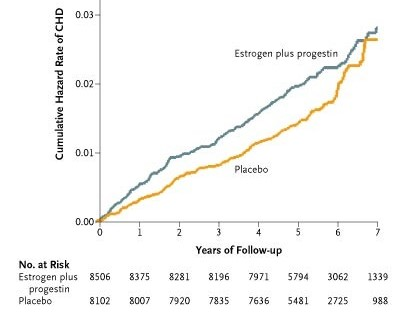
\includegraphics[width=\textwidth]{whi-on-mht-chd}
\end{minipage}
\hfill
\begin{minipage}[b]{0.42\linewidth}
{\small
\raggedright
\bi
\item
Curves of cumulative hazard approximate
the development of
cumulative risks $\pi_x(t)$ over time.
\item
In early years,
the curve of MHT runs on top, reflecting
higher hazard in that period.
\item
By 6-7 year, 
cumulative risks appear
to have reached same level.
\ei
}
\end{minipage}
\end{frame}

\begin{frame}
\frametitle{\large From hazards to causal contrasts of risk}
\bi
\item
A well-specified predictive model for hazards $\lambda(t|x,z)$ (e.g.
Cox or Poisson; suitably flexible) can, however, be used 
to estimate counterfactual cumulative risks  % $\pi^1(t)$ and $\pi^0(t)$:
%% \begin{center}
   $ \pi^x(t) = P\{ Y^{X=x}(t) \} = P\{ T^{X=x} \leq t \}, x=0,1 $. 
%% \end{center}
\pause
\medskip
\item
Suppose $Z$ blocks all non-causal paths. Then
{\bf counterfactual conditional hazards} 
$\lambda^x(t|Z=z)$ are identified by observable hazards $\lambda(t|x,z)$
%% $$ \lambda_x(t|Z=z) = \lim_{h\to 0} P\{ Y(t+h)=1| Y(t)=0, X=x, Z=z \}/h $$
%% \item
%% When $Z$ is continuous or vector-valued, a reasonable model for  $\lambda_x(t|Z=z)$
%% can often be built on e.g. Cox regression or its time-dep extensions.
%% \medskip
%% \item
%% Discrete-time hazards $P\{ Y(t_{k+1})=1| Y(t_k)=0, X=x, Z=z \}$ 
%% and binary models on these also used (e.g. by Hernan \& Robins).
%% \ei
%% \end{frame}

%% \begin{frame}
%% \frametitle{\large From hazards to causal contrasts of risk (cont'd)}

%% \bi
\pause
\medskip
\item When no competing events exist,
counterfactual $z$-specific risks $\pi^x(t|Z=z) = P\{ Y^{X=x}(t)|Z=z\} $ are identified from \\
factual $z$-conditional hazards 
\begin{center}
$ \pi^x(t|Z=z) = %%  \pi_x(t|Z=z) = 
    1 - \exp\left\{-\int_0^t \lambda(v|x,z)dv \right\} . $
\end{center}
\pause
\medskip		
\item		
Counterfactual marginal risks are obtained using the {g-formula}: \\
%% If $Z$ is discrete-valued, the formula is
$$ \pi^x(t) = \sum_z \pi_x(t|Z=z) P\{ Z=z \} . $$
%% \item
%% Thus, marginal risks are again weighted averages of 
%% the conditional ones, and use of g-formula corresponds to {\bf direct standardization}.
%% \medskip
%% {\small \item[NB.] For those more mathematically oriented: If $Z$ contains 
%% discrete and/or continuous variables, the 
%% sum is substituted by a {\bf Stieltjes-integral}, and the g-formula is technically expressed as
%% $\pi^x(t) = E_Z[\pi_x(t|Z)] = \int_z \pi_x(t| Z=z) dF(z), $
%% where $F(z)$ is the joint distribution function of $Z$ in the population.}

\ei


\end{frame}

\begin{frame}
\frametitle{\large Estimation of causal contrasts from time-to-event data}
\bi
\item
Various methods to estimate counterfactual % survival probabilities $1-\pi^x(t)$ and 
risks $\pi^{X=x}(t)$ and their contrasts 
({\small see \href{https://doi.org/10.1002/sim.9681}{\color{blue}Denz et al. 2023} })
\pause
 -- For instance
\medskip
\item[(a)] 
Fit a Cox model $\lambda(t|x_i, z_i) = \lambda_0(t)\exp(\beta x_i + \gamma^{T}z_i)$,
take estimates of coefficients and baseline cumulative hazard $\widehat\Lambda_0(t)$
% plus $\widehat\beta$ and $\widehat\gamma$, 
from which:
$$ % \begin{center}
 \widetilde{\pi}_i^{X_i=x}(t) = 1 - \exp \{ -\widehat\Lambda_0(t)\exp(\widehat\beta x + \widehat\gamma^{\small{\text{T}}} z_i) \}  .
$$ % \end{center}
Counterfactuals $ {\pi}^{X=x}(t)$ and contrasts are then estimated by g-formula.
\pause
\medskip
\item[(b)]
Get weights $W_i$ from an exposure model, fit Cox with ``intercept only'' 
specifying $X$ as a \texttt{strata()} variable and $W_i$:s as \texttt{weights}, and estimate $\widehat{\pi}^{X=x}(t)$
using \texttt{survfit()}, etc.
\pause
\medskip
\item Other: IPW Kaplan-Meier, use of pseudo-values, DR methods, \dots
\medskip
\item Competing event setting: additional complexities in defining and analysing causal contrasts
({\small see \href{https://doi.org/10.1007/s40471-020-00240-7}{\color{blue}Rudolph et al. 2020}, \ 
\href{https://doi.org/10.1002/sim.8471}{\color{blue}Young et al. 2020}}).    
\ei
\end{frame}


\end{document}

